\begin{figure*}
\begin{center}
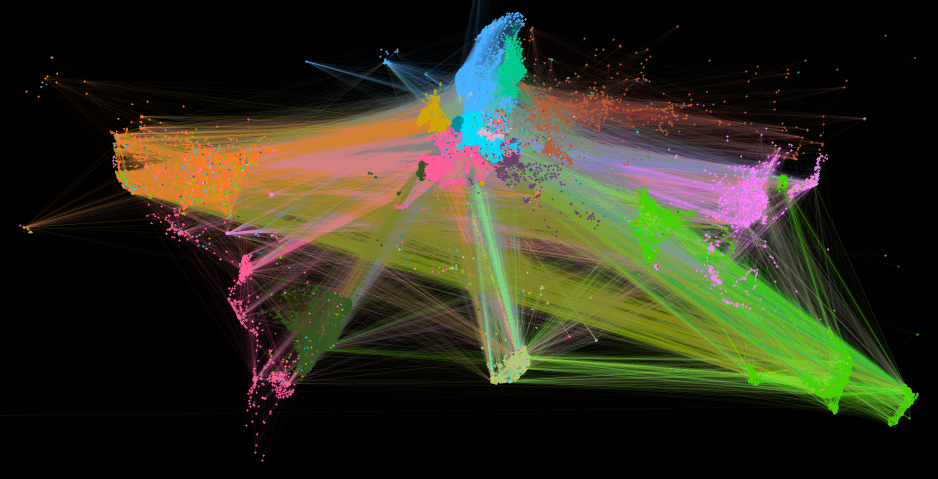
\includegraphics[width=.7\textwidth]{fig1.png}
\end{center}
\caption{Global network of interlocking directorates. Color indicates communities -- i.e. cities that do business together within each other more often than with others.}
\label{fig:fig1}
\end{figure*}


\section{Complexity theory}
\label{sec:complexity}
\input{\filenamebase.complexity}

\section{Research questions, concepts and propositions}
\label{sec:question}
\subsection{Interlocking directorates}
An important concept in this paper is `interlocking directorates'. An interlock corresponds to the link that is formed between two companies when a director affiliated with one organization sits on the board of directors of another organization ~\citep{Mizruchi1996}, or when two director from two firms sit together on the board of directors of a third firm. Importantly, while the interlock is a relationship between companies, it is created by individuals sitting in boards. This allows us to model the system as a bipartite (two-mode) network, and to analyze at the same time the importance of both companies and directors.

The concept of interlocking directorates is related to the corporate elite, part of the power elite. Mills~\cite{mills1957} defined the power elite as \textit{``those political, economic, and military circles, which as an intricate set of overlapping small but dominant groups share decisions having at least national consequences. Insofar as national events are decided, the power elite are those who decide them''}~\citep{mills1957}. Moreover, Mills determined that there is an `inner core' of the power elite involving individuals that are able to move from one seat of institutional power to another. In the context of corporations, this inner core corresponds to the corporate elite. A strength of using the concept of interlocking directorates as opposed to corporate elites is that we do not assume a priori characteristics of the elite. Corporate elites on the interlock network are the actors with high centralities values, as measured by network algorithms.

The effects of interlocks (or by extension the corporate elites) are still object to controversy. 
In the past decades, tens of papers have investigated the effect of interlocks in firm performance, innovation, acquisitions, mergers, capital growth, firm reputation, and adoption of structures and strategies (see for example review ~\cite{Mizruchi1996}).
However, only the spread of structures and strategies has been consistently associated to interlocks [refs].
We attribute this to bias to limitations in the data analysis.
Previous papers have focused on a small number of top companies (10--1000), 
many times restricting the study to only one sector or country. 
The result of this approach in a complex network is a misrepresentation of local patterns as the global patterns.
For instance, Mizruchi~\cite{Mizruchi1996} points out that if directors are appointed when the productivity of the firm is low (as a form of monitoring),
and directors decide to join boards that are performing well (as a form of career development),
the end result would be an inverted U shaped relationship between number of interlocks and firm performance. 
This model would explain why researchers [refs] have found positive and negative relationship between interlocks and performance,

In order to bring definite answers to the field we will study a large dataset comprising 200 million companies and 100 million directors (see \ref{sec:data}).
Our main research question is ``How is the interlocking directorates network structured in time and space, and what is their effect on investment and innovation''.
For the sake of brevity, we will focus here on the second part of the question ``what is the effect of interlocks on investment and innovation''. 
First, we will explore the concept of the product-service space (PSS), 
that determines how closely two sectors are depending on how many cities have companies in both sectors.
Economical development has been showed to depend on this concept~\citep{hidalgo2009}.
Secondly, we will determine how interlocks affect the evolution of the distribution of sectors within the city.
Thirdly, we will show what factors influence the presence of interlocks.
Our unit of analysis can be the company itself, the city, the country or the region. 
For clarity, because cities have became innovation hubs~\citep{Belderbos2014}, 
and because we do not want to impose a national structure on the data,
we will focus on the city level for the rest of the manuscript.


\subsection{Product-service space}
Cities and countries evolve economically (develop) by moving from producing simple products and services to specializing in more expensive ones -- a process referred to as `structural transformation'~\citep{smith1776, Romer1991,grossman1991,hidalgo2007}.
This transformation can be explained using differences in productive factors and technology (see ~\citep{hausmann2011} for a review).
In order to connect these differences to development, 
current models usually abstract from the product themselves and look at macro-economic indicators of productive factors and technology.
However, development occur when individual new products are created or existing ones improved,
and it is not clear that his models can explain the variability observed in countries with similar macro-economic indicators.
Moreover, the products that are developed depend on the current products being produced -- there is a relatedness between products.
Many explanation have been proposed for this, 
such as similar institutions, infrastructure, physical factors, technology, or some combination of those factors (see ~\cite{hidalgo2007} for a review).
Hidalgo, Hausman and Klinger~\cite{hidalgo2007, hausmann2011, Hausmann2006,hidalgo2009} developed the `product space' as a map of the relatedness between products,
where products are related if countries have competitive advantages respect to both products.
They showed that the product space capture information about the complexity of the set of capabilities available in a country, 
is strongly correlated with income per capita and predictive of future growth.
Furthermore, they proved that structural transformation at the country level occurs by moving from existing products to related products, 
where two products are related if they are closed in the `product space'.

In a world full of multi-nationals, innovation is happening at the city level~\citep{Belderbos2014}.
We adapt the `product-space' concept by focusing at relationships between company sectors at the city level,
instead of product categories at the country level.
Using cities allows us to explore not only products, but also services, thus we will define the `product-service space' (PSS). 
Moreover, focusing on city abstract for economic growth due to the number of companies in the city.
The subquestion here is: ``Does structural transformation at the city follows the product-service space''.
We expect to find comparable trends at the city level than Hidalgo, Hausman and Klinger found at the country level.
The structural transformation should follow the edges in the product-service space, 
and the diffusion process would correlate with gdp per capita in the city, 
and maybe with innovation, for which we can use the Innovation index \footnote{\url{http://www.innovation-cities.com/innovation-cities-index-2015-global/9609}}
or the number of patterns.
The causal argument is symmetrical from Hidalgo, Hausman and Klinger's argument~\cite{hidalgo2007, hausmann2011, Hausmann2006,hidalgo2009} but at the city level.
Cities require some underlying capabilities (infrastructure, education, institutions, human capital) to maintain specific companies,
and those capabilities are similar for sectors close together in the product-service space.
When a city acquire new capabilities, new products can be developed along the product-service space.
However, we are more interesting in understanding the role of interlocks in the process, 
thus we only intent to hint on causality.
Negative results would suggest an extreme globalization of the cities, 
where the benefit of having `in situ' capabilities is minimal.


%We will define the network as $PSS = (V, E)) $, where $V$ are the sectors according to NACE rev. 2 (e.g. C11 = Manufacture of beverages),
%and $E$ is the matrix of weights between sectors.


\subsection{Interlocks and the PSS}
%[Research subquestion herere]
We will analyze if interlocks are a predictor of diffusion between sectors in cities. 
Development itself influences the presence of interlocks.
Companies situated close geographically, or in places with similar language or colonial ties 
have greater chances to interlock [refs].
Since the establishment of companies in the city allow for greater possibilities of interlocks,
we expect a relationship between the PSS and the number of interlocks between sectors.
However it is not clear if interlocks are only a cause of development but also an effect.
Interlocks provide a communication channel between companies, 
and serve as a link for the spread of strategies and structures (refs).
For instance, [examples of previous research].
We hypothesize that interlocks serve as a communication channel for opportunities,
thus increasing investment and R\&D to sectors close in the PSS.
The increased investment and innovation has been linked to development~\citep{Romer1991,grossman1991,hidalgo2007}.
In a first step, we will test if interlocks affect the diffusion process in the PSS.
In a second step, we will analyze collaboration between companies using patent data to show if this diffusion process is mediated (at least partially) by innovation.

\subsubsection{Interlocks affect the PSS}
%[Research subquestion herere]
Figure ~\ref{fig:entropy} shows our approach. 
Given the number of companies in city A at time t (Fig. ~\ref{fig:entropy}A), 
we want to explain the evolution to time t+1 (Fig. ~\ref{fig:entropy}B).
~\cite{hidalgo2009} showed that this evolution (at the country level) is related to the `product space' (Fig. ~\ref{fig:entropy}C).
We can create a network of interlocks (Fig. ~\ref{fig:entropy}C),
where two sectors are connected if a director sits in companies from both sectors.
Importantly, the network of interlocks have relationships between sectors that are not present in Figure ~\ref{fig:entropy}A. 
This because interlocks are not restricted to the city itself.
A director can sit in the banking sector in city A and in the IT sector in city B, even if there are no IT companies in city A.
Our research question here is then ``To what extent do interlocks increase the diffusion rates in the PSS''.


\begin{figure}
\begin{center}
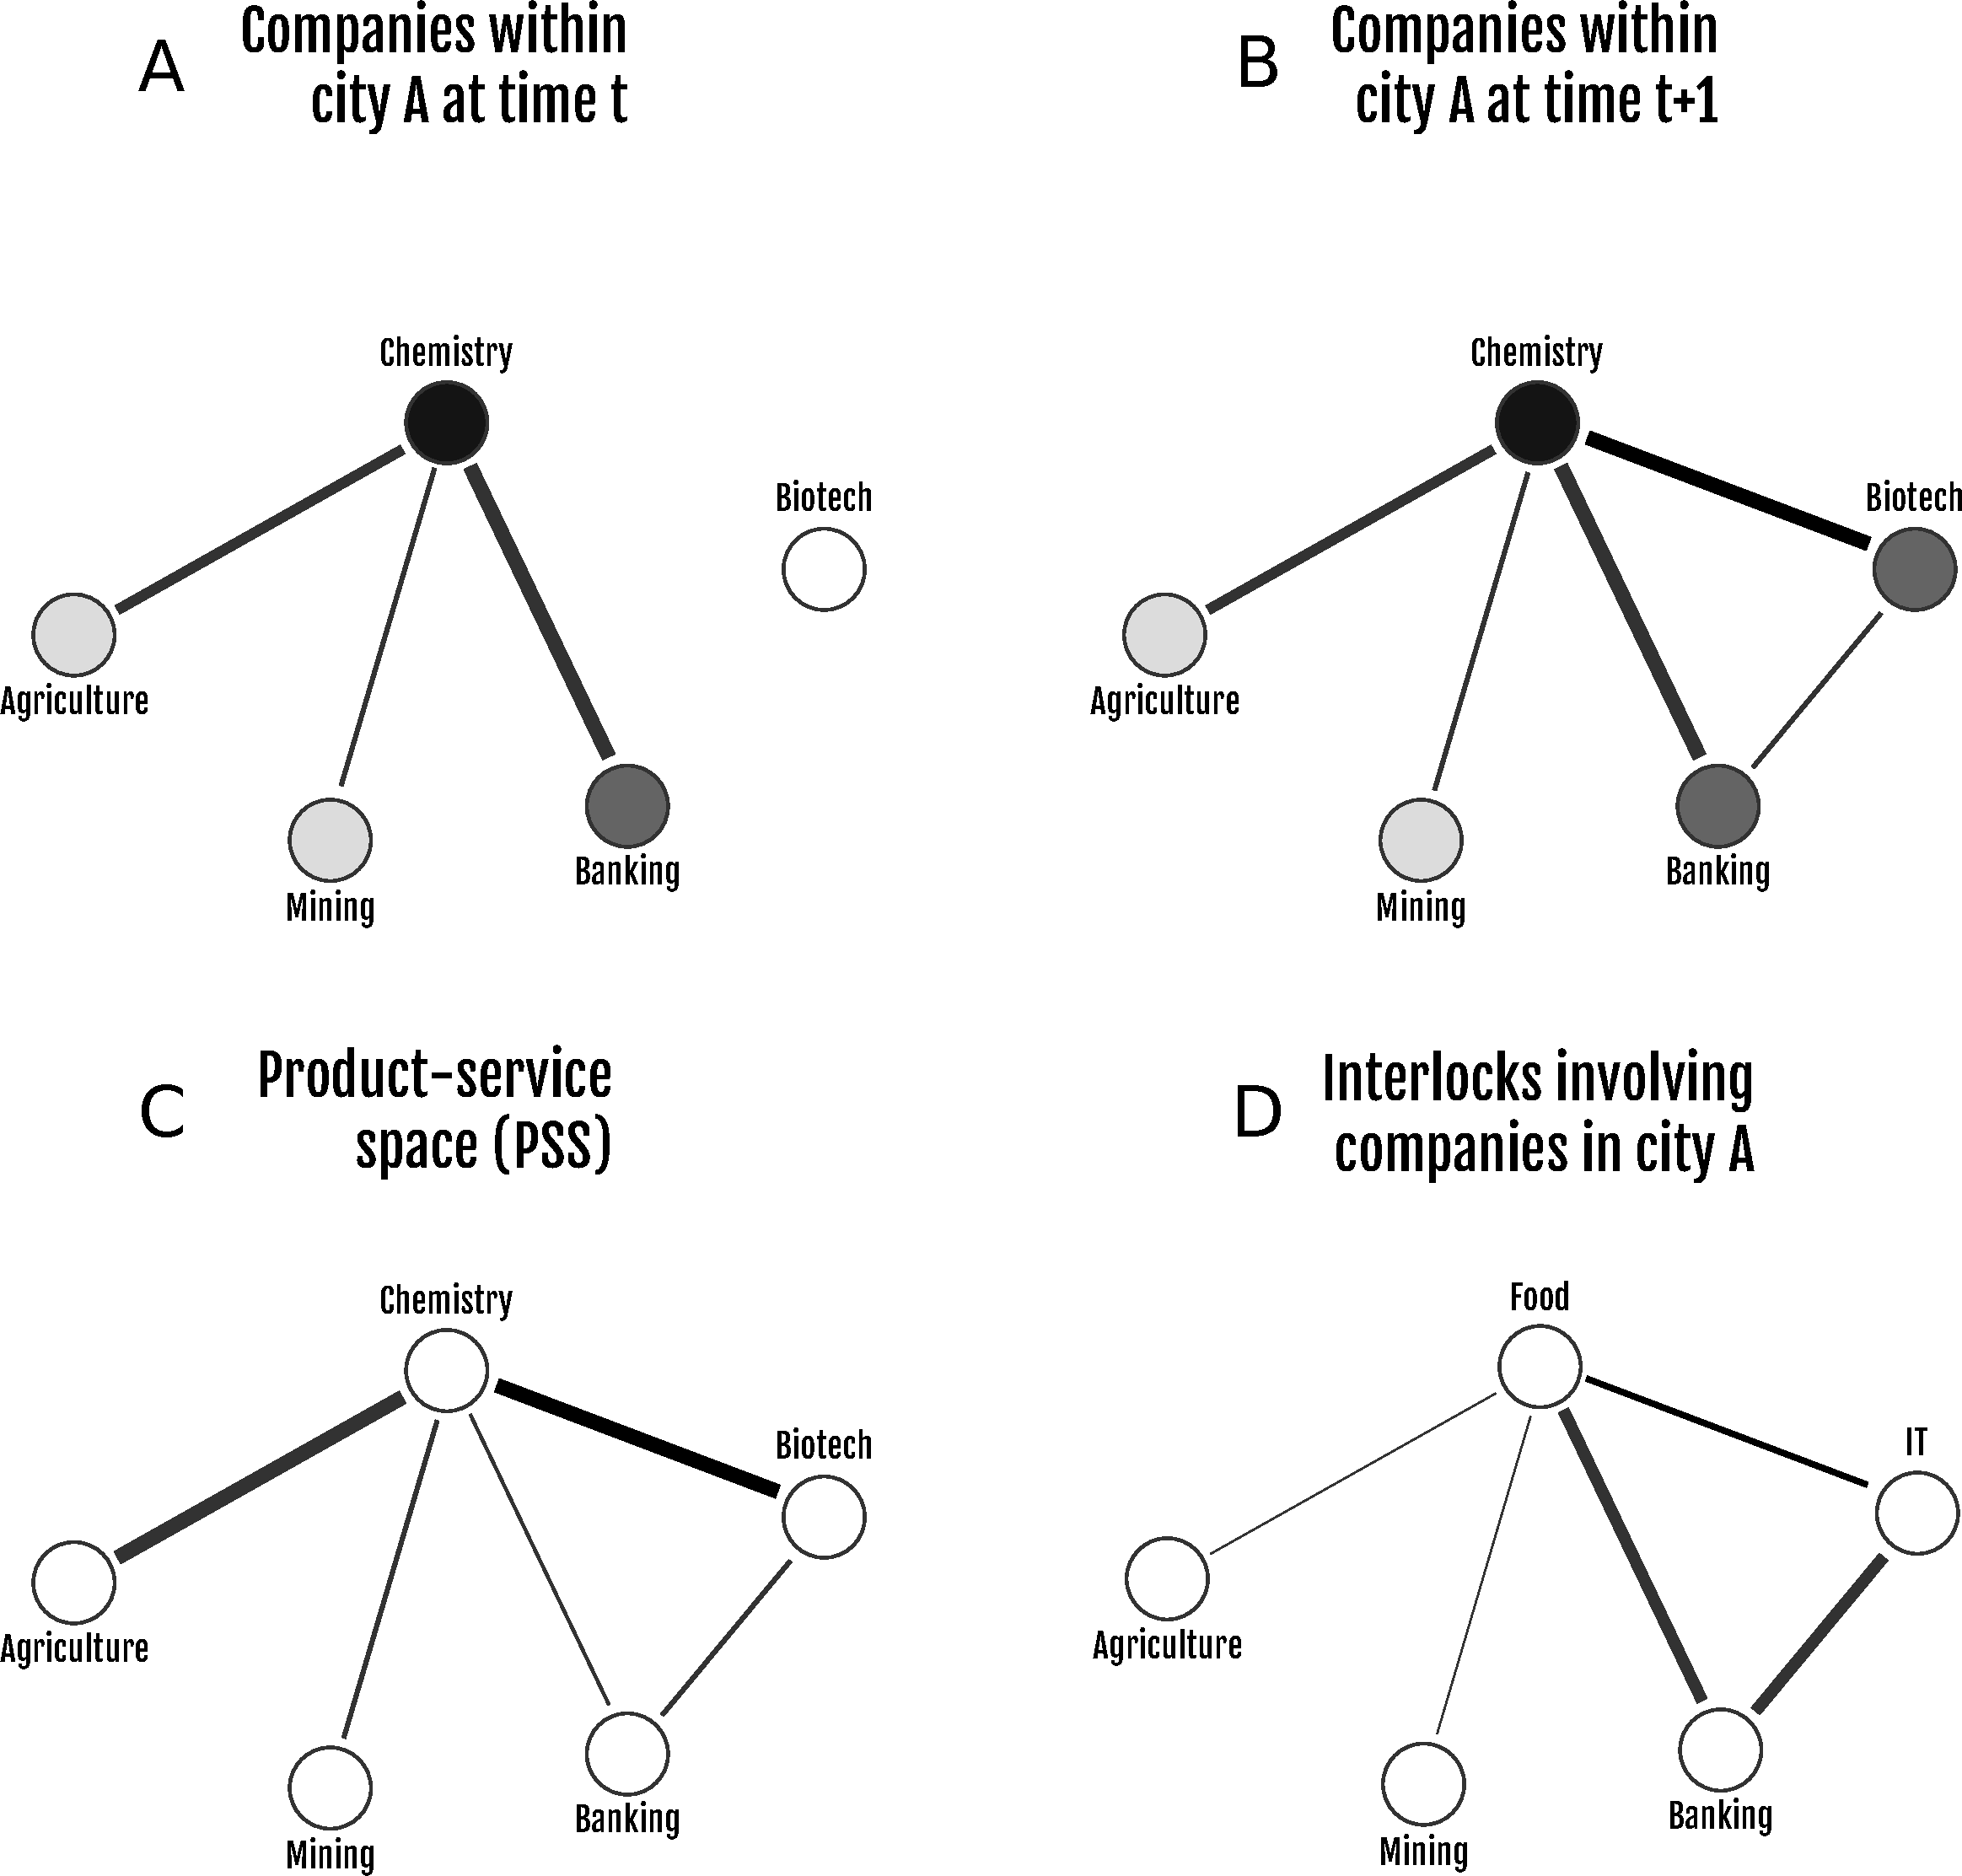
\includegraphics[width=.5\textwidth]{entropy.pdf}
\caption{.}
\label{fig:entropy}
\end{center}
\end{figure}

One method to study if interlocks are predictors of the diffusion process is conditional entropy $H(X|Y)$.
The conditional entropy  $H(Companies_{t_1}|Companies_{t_0})$ quantifies how much information we need to define the structure of the network at time 1 knowing the structure at time 0. 
If the network of interlocks between sectors affect the network we will find that $H(Companies_{t_1}|Companies_{t_0},Interlocks_{t_0}) < H(Companies_{t_1}|Companies_{t_0})$.


There are several problems with this approach.
Firstly, we have explained that development creates interlocks (endogeneity problem).
The use of longitudinal data allows us to quantify the effect of interlocks on development,
independently of the effect of development on interlocks.
Secondly, there is a chance of self-selection bias.
Companies that want to develop to a new sector may create interlocks with that sector beforehand.
However, if this is true, interlocks would also facilitate diffusion.
Finally, a most important bias is omitted variable bias.
If there is an underlying mechanism that produces the interlock at $time_1$ and the diffusion at $time_2$, 
we would find a false effect of interlocks on the diffusion process.
For example, cities that are developing fast (for whatever reason) may attract more interlocks than those who are not developing.
In order to investigate this possibility, we need to control for city economic indicators, such as infrastructure, resources, education, population density.
Other variables to control are sector size, number of companies, country indicators and type of interlocks (within city vs between cities).
We can create random models using the product-service space and these variables to investigate their effect

\subsubsection{Interlocks affect the company space (at least) through innovation}
The subquestion corresponding to this subsection is ``Do interlocks foster collaboration between companies and innovation?''.
%In the case of , 
%- Innovation has become one of the key strategies of the firm for gaining competitive advantage (Hitt et al., 1996), expanding market share (Franko, 1989) and increasing firm performance (Morbey, 1988



\subsection{Which factors affect interlocks}
\label{sec:factors}
The literature for the factors influencing interlock creation is more consistent.
Geographical distance, colony history, language, education and social networks have been pointed as factors
influencing the presence of interlocks [refs].
Time allowing, we will explore this idea at the micro-scale using generative models such as ERGMs,
which allow to control for network effects such as transitivity -- i.e. the probability that there is an interlock A--C if there are interlocks A--B and B--C is increased, and should be controlled.


\subsection{Other projects}
The data allow for the exploration of other projects, such as:
(i) Description of inequality.
(ii) Homogenization of coordinated and liberal market economies.
(iii) Quantify the independence of a given sector (e.g. food).
(iv) Measure the transference of power from domestic corporation to transnational corporations.
(v) Network motifs, which combination of interlocks between sectors are more likely than random.

